\documentclass[twoside]{article}

% Packages required by doxygen
\usepackage{fixltx2e}
\usepackage{calc}
\usepackage{doxygen}
\usepackage[export]{adjustbox} % also loads graphicx
\usepackage{graphicx}
\usepackage[utf8]{inputenc}
\usepackage{makeidx}
\usepackage{multicol}
\usepackage{multirow}
\PassOptionsToPackage{warn}{textcomp}
\usepackage{textcomp}
\usepackage[nointegrals]{wasysym}
\usepackage[table]{xcolor}

% Font selection
\usepackage[T1]{fontenc}
\usepackage[scaled=.90]{helvet}
\usepackage{courier}
\usepackage{amssymb}
\usepackage{sectsty}
\renewcommand{\familydefault}{\sfdefault}
\allsectionsfont{%
  \fontseries{bc}\selectfont%
  \color{darkgray}%
}
\renewcommand{\DoxyLabelFont}{%
  \fontseries{bc}\selectfont%
  \color{darkgray}%
}
\newcommand{\+}{\discretionary{\mbox{\scriptsize$\hookleftarrow$}}{}{}}

% Page & text layout
\usepackage{geometry}
\geometry{%
  a4paper,%
  top=2.5cm,%
  bottom=2.5cm,%
  left=2.5cm,%
  right=2.5cm%
}
\tolerance=750
\hfuzz=15pt
\hbadness=750
\setlength{\emergencystretch}{15pt}
\setlength{\parindent}{0cm}
\setlength{\parskip}{3ex plus 2ex minus 2ex}
\makeatletter
\renewcommand{\paragraph}{%
  \@startsection{paragraph}{4}{0ex}{-1.0ex}{1.0ex}{%
    \normalfont\normalsize\bfseries\SS@parafont%
  }%
}
\renewcommand{\subparagraph}{%
  \@startsection{subparagraph}{5}{0ex}{-1.0ex}{1.0ex}{%
    \normalfont\normalsize\bfseries\SS@subparafont%
  }%
}
\makeatother

% Headers & footers
\usepackage{fancyhdr}
\pagestyle{fancyplain}
\fancyhead[LE]{\fancyplain{}{\bfseries\thepage}}
\fancyhead[CE]{\fancyplain{}{}}
\fancyhead[RE]{\fancyplain{}{\bfseries\leftmark}}
\fancyhead[LO]{\fancyplain{}{\bfseries\rightmark}}
\fancyhead[CO]{\fancyplain{}{}}
\fancyhead[RO]{\fancyplain{}{\bfseries\thepage}}
\fancyfoot[LE]{\fancyplain{}{}}
\fancyfoot[CE]{\fancyplain{}{}}
\fancyfoot[RE]{\fancyplain{}{\bfseries\scriptsize Generated by Doxygen }}
\fancyfoot[LO]{\fancyplain{}{\bfseries\scriptsize Generated by Doxygen }}
\fancyfoot[CO]{\fancyplain{}{}}
\fancyfoot[RO]{\fancyplain{}{}}
\renewcommand{\footrulewidth}{0.4pt}
\renewcommand{\sectionmark}[1]{%
  \markright{\thesection\ #1}%
}

% Indices & bibliography
\usepackage{natbib}
\usepackage[titles]{tocloft}
\setcounter{tocdepth}{3}
\setcounter{secnumdepth}{5}
\makeindex

% Hyperlinks (required, but should be loaded last)
\usepackage{ifpdf}
\ifpdf
  \usepackage[pdftex,pagebackref=true]{hyperref}
\else
  \usepackage[ps2pdf,pagebackref=true]{hyperref}
\fi
\hypersetup{%
  colorlinks=true,%
  linkcolor=blue,%
  citecolor=blue,%
  unicode%
}

% Custom commands
\newcommand{\clearemptydoublepage}{%
  \newpage{\pagestyle{empty}\cleardoublepage}%
}

\usepackage{caption}
\captionsetup{labelsep=space,justification=centering,font={bf},singlelinecheck=off,skip=4pt,position=top}

%===== C O N T E N T S =====

\begin{document}

% Titlepage & ToC
\hypersetup{pageanchor=false,
             bookmarksnumbered=true,
             pdfencoding=unicode
            }
\pagenumbering{roman}
\begin{titlepage}
\vspace*{7cm}
\begin{center}%
{\Large P\+A04-\/\+Timer }\\
\vspace*{1cm}
{\large Generated by Doxygen 1.8.11}\\
\end{center}
\end{titlepage}
\tableofcontents
\pagenumbering{arabic}
\hypersetup{pageanchor=true}

%--- Begin generated contents ---
\section{Main Page}
\label{index}\hypertarget{index}{}This project contains the following items -\/create an implementation of the Weighted Graph A\+DT usin ga vertex list and an adjacency matrix. -\/\+Develop a routine that finds the shorted path between each pair of vertices in a graph. -\/add vertex coloring and implement a function that checks whether a graph has a proper coloring. -\/investiate the four color theorem by generating a graph for which no proper coloring can be creating using less than five colors. 
\section{Hierarchical Index}
\subsection{Class Hierarchy}
This inheritance list is sorted roughly, but not completely, alphabetically\+:\begin{DoxyCompactList}
\item \contentsline{section}{Greater$<$ Key\+Type $>$}{\pageref{class_greater}}{}
\item \contentsline{section}{Heap$<$ Data\+Type, Key\+Type, Comparator $>$}{\pageref{class_heap}}{}
\item \contentsline{section}{Heap$<$ Data\+Type $>$}{\pageref{class_heap}}{}
\begin{DoxyCompactList}
\item \contentsline{section}{Priority\+Queue$<$ Data\+Type, Key\+Type, Comparator $>$}{\pageref{class_priority_queue}}{}
\end{DoxyCompactList}
\item \contentsline{section}{Less$<$ Key\+Type $>$}{\pageref{class_less}}{}
\item \contentsline{section}{Less$<$ int $>$}{\pageref{class_less}}{}
\item \contentsline{section}{Task\+Data}{\pageref{struct_task_data}}{}
\item \contentsline{section}{Test\+Data}{\pageref{class_test_data}}{}
\item \contentsline{section}{Test\+Data\+Item$<$ Key\+Type $>$}{\pageref{class_test_data_item}}{}
\end{DoxyCompactList}

\section{Class Index}
\subsection{Class List}
Here are the classes, structs, unions and interfaces with brief descriptions\+:\begin{DoxyCompactList}
\item\contentsline{section}{\hyperlink{classbinary_search}{binary\+Search} }{\pageref{classbinary_search}}{}
\item\contentsline{section}{\hyperlink{classlinear_search}{linear\+Search} }{\pageref{classlinear_search}}{}
\item\contentsline{section}{\hyperlink{class_search}{Search} }{\pageref{class_search}}{}
\item\contentsline{section}{\hyperlink{class_s_t_l_search}{S\+T\+L\+Search} }{\pageref{class_s_t_l_search}}{}
\item\contentsline{section}{\hyperlink{class_test_vector}{Test\+Vector} }{\pageref{class_test_vector}}{}
\item\contentsline{section}{\hyperlink{class_timer}{Timer} }{\pageref{class_timer}}{}
\end{DoxyCompactList}

\section{File Index}
\subsection{File List}
Here is a list of all files with brief descriptions\+:\begin{DoxyCompactList}
\item\contentsline{section}{\hyperlink{okay_8cpp}{okay.\+cpp} }{\pageref{okay_8cpp}}{}
\item\contentsline{section}{\hyperlink{_rush_hour_8cpp}{Rush\+Hour.\+cpp} }{\pageref{_rush_hour_8cpp}}{}
\end{DoxyCompactList}

\section{Class Documentation}
\hypertarget{classbinary_search}{}\subsection{binary\+Search Class Reference}
\label{classbinary_search}\index{binary\+Search@{binary\+Search}}
Inheritance diagram for binary\+Search\+:\begin{figure}[H]
\begin{center}
\leavevmode
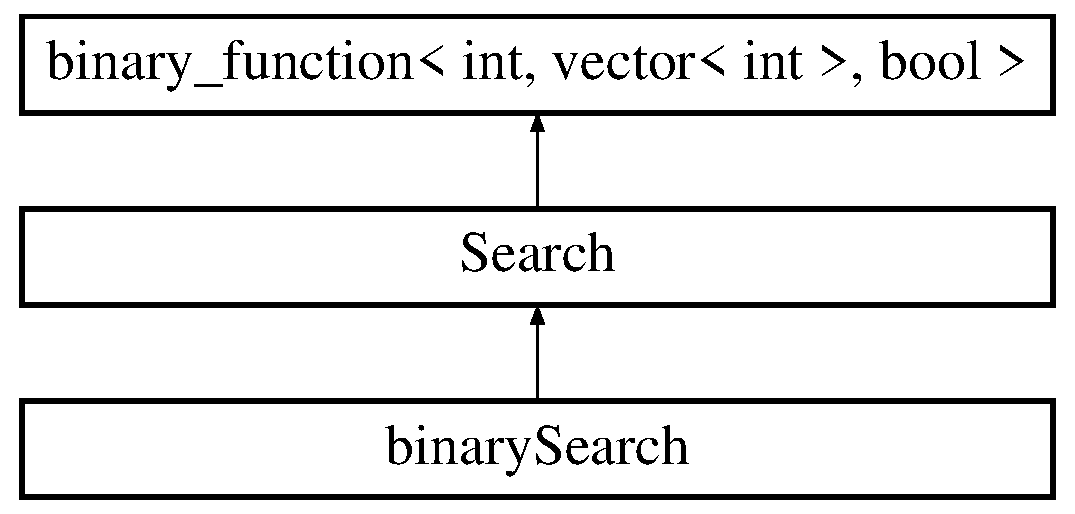
\includegraphics[height=3.000000cm]{classbinary_search}
\end{center}
\end{figure}
\subsubsection*{Public Member Functions}
\begin{DoxyCompactItemize}
\item 
bool {\bfseries operator()} (int search\+Value, const vector$<$ int $>$ \&keys) const \hypertarget{classbinary_search_a8e145edfb29183d7e1b265bd4cf4293f}{}\label{classbinary_search_a8e145edfb29183d7e1b265bd4cf4293f}

\end{DoxyCompactItemize}


The documentation for this class was generated from the following file\+:\begin{DoxyCompactItemize}
\item 
search.\+cpp\end{DoxyCompactItemize}

\hypertarget{classlinear_search}{}\subsection{linear\+Search Class Reference}
\label{classlinear_search}\index{linear\+Search@{linear\+Search}}
Inheritance diagram for linear\+Search\+:\begin{figure}[H]
\begin{center}
\leavevmode
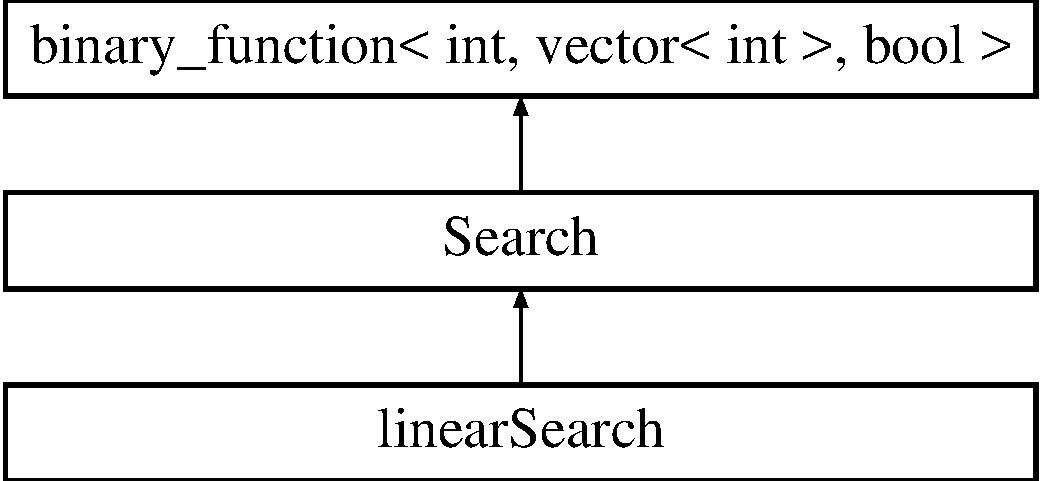
\includegraphics[height=3.000000cm]{classlinear_search}
\end{center}
\end{figure}
\subsubsection*{Public Member Functions}
\begin{DoxyCompactItemize}
\item 
bool {\bfseries operator()} (int search\+Value, const vector$<$ int $>$ \&keys) const \hypertarget{classlinear_search_a447bc4f724457f1786dc36c10626bfa8}{}\label{classlinear_search_a447bc4f724457f1786dc36c10626bfa8}

\end{DoxyCompactItemize}


The documentation for this class was generated from the following file\+:\begin{DoxyCompactItemize}
\item 
search.\+cpp\end{DoxyCompactItemize}

\hypertarget{class_search}{}\subsection{Search Class Reference}
\label{class_search}\index{Search@{Search}}
Inheritance diagram for Search\+:\begin{figure}[H]
\begin{center}
\leavevmode
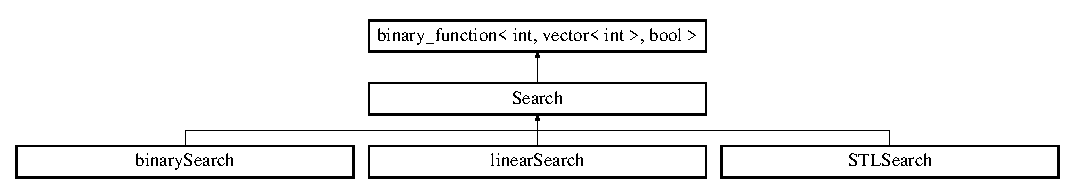
\includegraphics[height=2.153846cm]{class_search}
\end{center}
\end{figure}
\subsubsection*{Private Member Functions}
\begin{DoxyCompactItemize}
\item 
virtual bool {\bfseries operator()} (int search\+Value, const vector$<$ int $>$ \&keys) const =0\hypertarget{class_search_a3aef7c0a6c68824120046ae7ca8f8d48}{}\label{class_search_a3aef7c0a6c68824120046ae7ca8f8d48}

\end{DoxyCompactItemize}


The documentation for this class was generated from the following file\+:\begin{DoxyCompactItemize}
\item 
search.\+cpp\end{DoxyCompactItemize}

\hypertarget{class_s_t_l_search}{}\subsection{S\+T\+L\+Search Class Reference}
\label{class_s_t_l_search}\index{S\+T\+L\+Search@{S\+T\+L\+Search}}
Inheritance diagram for S\+T\+L\+Search\+:\begin{figure}[H]
\begin{center}
\leavevmode
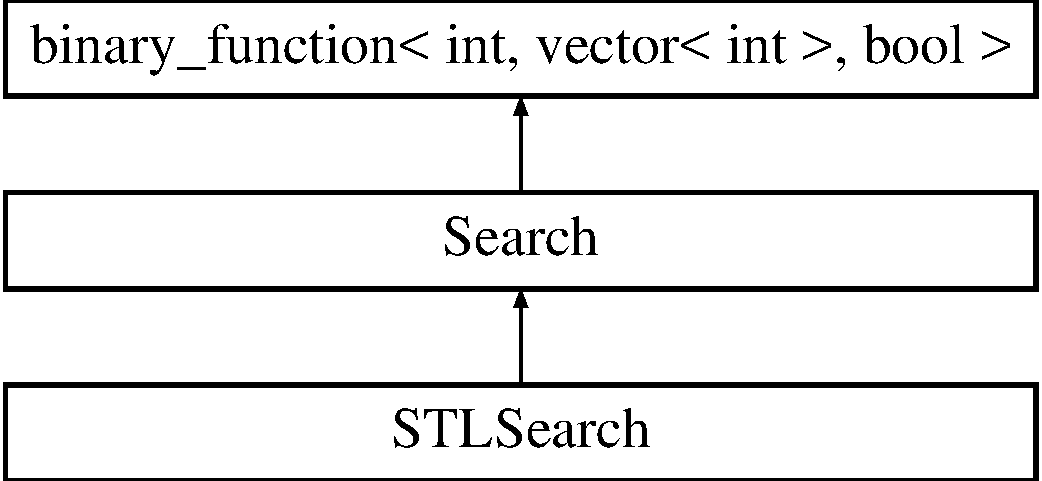
\includegraphics[height=3.000000cm]{class_s_t_l_search}
\end{center}
\end{figure}
\subsubsection*{Public Member Functions}
\begin{DoxyCompactItemize}
\item 
bool {\bfseries operator()} (int search\+Value, const vector$<$ int $>$ \&keys) const \hypertarget{class_s_t_l_search_a0f3684e33bd5e47317ab5a94d6f52dba}{}\label{class_s_t_l_search_a0f3684e33bd5e47317ab5a94d6f52dba}

\end{DoxyCompactItemize}


The documentation for this class was generated from the following file\+:\begin{DoxyCompactItemize}
\item 
search.\+cpp\end{DoxyCompactItemize}

\hypertarget{class_test_vector}{}\subsection{Test\+Vector Class Reference}
\label{class_test_vector}\index{Test\+Vector@{Test\+Vector}}
\subsubsection*{Public Member Functions}
\begin{DoxyCompactItemize}
\item 
{\bfseries Test\+Vector} (int size)\hypertarget{class_test_vector_abf540180761043bb7ac2665e147bdd33}{}\label{class_test_vector_abf540180761043bb7ac2665e147bdd33}

\item 
{\bfseries Test\+Vector} (const \hyperlink{class_test_vector}{Test\+Vector} \&rhs)\hypertarget{class_test_vector_a4a48046f67cc822ce9a6907f022a5d61}{}\label{class_test_vector_a4a48046f67cc822ce9a6907f022a5d61}

\item 
\hyperlink{class_test_vector}{Test\+Vector} \& {\bfseries operator++} ()\hypertarget{class_test_vector_a8d4a95de7e0e9985ffcd86280efb631d}{}\label{class_test_vector_a8d4a95de7e0e9985ffcd86280efb631d}

\item 
\hyperlink{class_test_vector}{Test\+Vector} {\bfseries operator++} (int ignored)\hypertarget{class_test_vector_a1b9640623055cd4618606cd2f0ed08b3}{}\label{class_test_vector_a1b9640623055cd4618606cd2f0ed08b3}

\item 
int {\bfseries operator\mbox{[}$\,$\mbox{]}} (int loc) const \hypertarget{class_test_vector_ae244371b88cb0ab127a877e5206b7ed8}{}\label{class_test_vector_ae244371b88cb0ab127a877e5206b7ed8}

\end{DoxyCompactItemize}
\subsubsection*{Private Attributes}
\begin{DoxyCompactItemize}
\item 
vector$<$ int $>$ {\bfseries values}\hypertarget{class_test_vector_a5f1f8a4c55c4ce94b93b645c1813efc1}{}\label{class_test_vector_a5f1f8a4c55c4ce94b93b645c1813efc1}

\end{DoxyCompactItemize}


The documentation for this class was generated from the following files\+:\begin{DoxyCompactItemize}
\item 
testvector.\+h\item 
testvector.\+cpp\end{DoxyCompactItemize}

\hypertarget{class_timer}{}\subsection{Timer Class Reference}
\label{class_timer}\index{Timer@{Timer}}
\subsubsection*{Public Member Functions}
\begin{DoxyCompactItemize}
\item 
\hyperlink{class_timer_a5f16e8da27d2a5a5242dead46de05d97}{Timer} ()
\item 
void \hyperlink{class_timer_a3a8b5272198d029779dc9302a54305a8}{start} ()  throw (runtime\+\_\+error)
\item 
void \hyperlink{class_timer_a63f0eb44b27402196590a03781515dba}{stop} ()  throw (logic\+\_\+error)
\item 
double \hyperlink{class_timer_ad306e18f8d8a0296e001683f92d7f86e}{get\+Elapsed\+Time} () const   throw (logic\+\_\+error)
\end{DoxyCompactItemize}
\subsubsection*{Private Attributes}
\begin{DoxyCompactItemize}
\item 
struct timeval {\bfseries begin\+Time}\hypertarget{class_timer_a2066f4c22ec30af19681442f4f57bc28}{}\label{class_timer_a2066f4c22ec30af19681442f4f57bc28}

\item 
struct timeval {\bfseries duration}\hypertarget{class_timer_a9bdb26b09da69f87a7af343e9a229c65}{}\label{class_timer_a9bdb26b09da69f87a7af343e9a229c65}

\item 
bool {\bfseries timer\+Was\+Started}\hypertarget{class_timer_aea3956cc379872b4b0a93a1ece66ce4d}{}\label{class_timer_aea3956cc379872b4b0a93a1ece66ce4d}

\end{DoxyCompactItemize}


\subsubsection{Constructor \& Destructor Documentation}
\index{Timer@{Timer}!Timer@{Timer}}
\index{Timer@{Timer}!Timer@{Timer}}
\paragraph[{\texorpdfstring{Timer()}{Timer()}}]{\setlength{\rightskip}{0pt plus 5cm}Timer\+::\+Timer (
\begin{DoxyParamCaption}
{}
\end{DoxyParamCaption}
)}\hypertarget{class_timer_a5f16e8da27d2a5a5242dead46de05d97}{}\label{class_timer_a5f16e8da27d2a5a5242dead46de05d97}
This function will create a timer class using the constructor. This function is the default constructor of the \hyperlink{class_timer}{Timer} class.

This function will be used specifically to initialize a \hyperlink{class_timer}{Timer} class with all of the private struct values to be set to and the boolean timer\+Was\+Started to false since it was never started.


\begin{DoxyParams}{Parameters}
{\em none.} & \\
\hline
\end{DoxyParams}
\begin{DoxyReturn}{Returns}
This function does not return anything.
\end{DoxyReturn}
\begin{DoxyPrecond}{Precondition}
none. 
\end{DoxyPrecond}
\begin{DoxyPostcond}{Postcondition}
The timer class will be intialized to have a begin\+Time and duration struct with the time for both of their tv\+\_\+sec and tv\+\_\+usec members set to 0. The boolean timer\+Was\+Started will be set to false since the time is not started. It is just initialized. 
\end{DoxyPostcond}


\subsubsection{Member Function Documentation}
\index{Timer@{Timer}!get\+Elapsed\+Time@{get\+Elapsed\+Time}}
\index{get\+Elapsed\+Time@{get\+Elapsed\+Time}!Timer@{Timer}}
\paragraph[{\texorpdfstring{get\+Elapsed\+Time() const }{getElapsedTime() const }}]{\setlength{\rightskip}{0pt plus 5cm}double Timer\+::get\+Elapsed\+Time (
\begin{DoxyParamCaption}
{}
\end{DoxyParamCaption}
) const throw  logic\+\_\+error) }\hypertarget{class_timer_ad306e18f8d8a0296e001683f92d7f86e}{}\label{class_timer_ad306e18f8d8a0296e001683f92d7f86e}
This function is the \hyperlink{class_timer_ad306e18f8d8a0296e001683f92d7f86e}{get\+Elapsed\+Time()} function for the \hyperlink{class_timer}{Timer} class.

This function takes members of the duration structure and calculates the elapsed time and returns it as a double. This function will throw a logic error if timer\+Was\+Started is set to true because it is then assumed that the timer is still running at that point.


\begin{DoxyParams}{Parameters}
{\em none.} & \\
\hline
\end{DoxyParams}
\begin{DoxyReturn}{Returns}
This function returns a double that represents the amount of time that has passed since the timer was stopped and started.
\end{DoxyReturn}
\begin{DoxyPrecond}{Precondition}
timer\+Was\+Started is set to false. 
\end{DoxyPrecond}
\begin{DoxyPostcond}{Postcondition}
The function takes the tv\+\_\+sec and tv\+\_\+usec values from the duration structure in the timer class and adds it together and stores it in a local double variable. The function then divides the value of the local variable by 10$^\wedge$6. The function will then return the elapsed\+Time local variable since it stores the value of the time that has passed. 
\end{DoxyPostcond}
\index{Timer@{Timer}!start@{start}}
\index{start@{start}!Timer@{Timer}}
\paragraph[{\texorpdfstring{start()}{start()}}]{\setlength{\rightskip}{0pt plus 5cm}void Timer\+::start (
\begin{DoxyParamCaption}
{}
\end{DoxyParamCaption}
) throw  runtime\+\_\+error) }\hypertarget{class_timer_a3a8b5272198d029779dc9302a54305a8}{}\label{class_timer_a3a8b5272198d029779dc9302a54305a8}
This function is the \hyperlink{class_timer_a3a8b5272198d029779dc9302a54305a8}{start()} function of the \hyperlink{class_timer}{Timer} class.

This function will be used specifically to initialize the timer start for the timer class. The function throws a runtime\+\_\+error saying the timer was already started since if the timer was already started, there is nothing left to start.


\begin{DoxyParams}{Parameters}
{\em none.} & \\
\hline
\end{DoxyParams}
\begin{DoxyReturn}{Returns}
This function does not return anything.
\end{DoxyReturn}
\begin{DoxyPrecond}{Precondition}
timer\+Was\+Started should be set to false. 
\end{DoxyPrecond}
\begin{DoxyPostcond}{Postcondition}
The timer class will intialize the structure times to start with the use of gettimeofday function given by a given library in the header file. the function will set the timer\+Was\+Started variable to true since the timer will now start recording. 
\end{DoxyPostcond}
\index{Timer@{Timer}!stop@{stop}}
\index{stop@{stop}!Timer@{Timer}}
\paragraph[{\texorpdfstring{stop()}{stop()}}]{\setlength{\rightskip}{0pt plus 5cm}void Timer\+::stop (
\begin{DoxyParamCaption}
{}
\end{DoxyParamCaption}
) throw  logic\+\_\+error) }\hypertarget{class_timer_a63f0eb44b27402196590a03781515dba}{}\label{class_timer_a63f0eb44b27402196590a03781515dba}
This function is the \hyperlink{class_timer_a63f0eb44b27402196590a03781515dba}{stop()} function of the \hyperlink{class_timer}{Timer} class.

This function will be used specifically to stop the time for the timer class. The function will throw a logic error is timer was never started because there would be nothing to stop if timer was never started.


\begin{DoxyParams}{Parameters}
{\em none.} & \\
\hline
\end{DoxyParams}
\begin{DoxyReturn}{Returns}
This function does not return anything.
\end{DoxyReturn}
\begin{DoxyPrecond}{Precondition}
timer\+Was\+Started should be set to true. 
\end{DoxyPrecond}
\begin{DoxyPostcond}{Postcondition}
The timer class will stop the timer within the structure by using gettimeofday function again. It will then take the difference of the tv\+\_\+sec and tv\+\_\+usec variables from the begin\+Time structure of the class and the stop structure that was created within this function. The function will take the difference of tv\+\_\+sec and multiply it by 10$^\wedge$6 and store it to the tv\+\_\+sec member of the duration structure in the timer class. The function also takes the difference of the tv\+\_\+usec and store it to the tv\+\_\+usec member of the duration structure in the timer class. 
\end{DoxyPostcond}


The documentation for this class was generated from the following files\+:\begin{DoxyCompactItemize}
\item 
Timer.\+h\item 
\hyperlink{_timer_8cpp}{Timer.\+cpp}\item 
Timer.\+cs\end{DoxyCompactItemize}

\section{File Documentation}
\hypertarget{_timer_8cpp}{}\subsection{Timer.\+cpp File Reference}
\label{_timer_8cpp}\index{Timer.\+cpp@{Timer.\+cpp}}


This program will implement a timer to test multiple sort, searches, constructor and increment tests.  


{\ttfamily \#include $<$iostream$>$}\\*
{\ttfamily \#include \char`\"{}Timer.\+h\char`\"{}}\\*


\subsubsection{Detailed Description}
This program will implement a timer to test multiple sort, searches, constructor and increment tests. 

\begin{DoxyAuthor}{Author}
Kripash Shrestha 
\end{DoxyAuthor}
\begin{DoxyVersion}{Version}
1.\+0
\end{DoxyVersion}
The specifications of the program are instructed and documented on Lab 13 Performance Evaluation of C++ Data Structures\+: A Laboratory Course Third Edition by Brandle, Geisler, Roberge and Whittington \begin{DoxyDate}{Date}
Wednesday, September 26, 2017 
\end{DoxyDate}

%--- End generated contents ---

% Index
\newpage
\phantomsection
\clearemptydoublepage
\addcontentsline{toc}{section}{Index}
\printindex

\end{document}
